 \documentclass{report}
 
\usepackage[utf8]{inputenc} 
\usepackage[T1]{fontenc}      
\usepackage[top=2.0cm, bottom=3cm, left=3.0cm, right=3.0cm]{geometry}
\usepackage{graphicx}
\usepackage{wrapfig}
\usepackage{amsmath,esint }
\usepackage{amssymb}
\graphicspath{{figures/}{../figures}}

\newcommand*\dif{\mathop{}\!\mathrm{d}}
\newcommand*\diver{\mathop{}\!\mathrm{div}}
\newcommand*\grad{\mathop{}\!\mathrm{grad}}

\begin{document}

\section*{Questions de cours}

\begin{itemize}

	\item[$\ast$] Un cylindre (rayon $R$, longueur $L$, $R\ll L$) de matériau ferromagnétique dur est enroulé sur tout sa longueur par $N$ spires, d'un fil parcouru d'un courant $I$. Donner l'allure des champs $\vec{B}/\mu_0$, $\vec{H}$ et $\vec{M}$ le long de l'axe du cylindre (noté $z$). On supposera que l'aimatation est uniforme dans tout le matériau. On s'intéressera en particulier au cas où $B>0$ et $H<0$.
	
		\begin{figure}[h!]
	\centering
		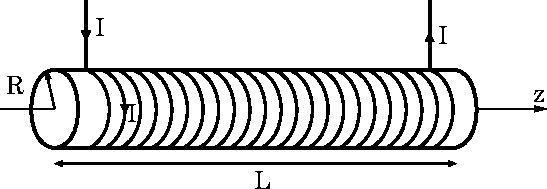
\includegraphics[scale=0.7]{ferro.pdf}
	\end{figure}	
	
	\item[$\ast$] Un cylindre (rayon $R$, longueur $L$, $R\ll L$) de matériau ferromagnétique doux est enroulé sur tout sa longueur par $N$ spires, d'un fil parcouru d'un courant $i(t)$. Quel est l'inductance $L$ du circuit ? Même question dans le cas d'un ferromagnétique dur. 
	
	\begin{figure}[h!]
	\centering
		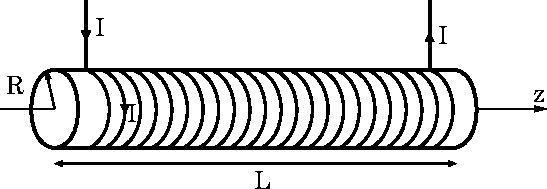
\includegraphics[scale=0.7]{ferro.pdf}
	\end{figure}	
	
	\item[$\ast$] Décrire le modèle du transformateur parfait.
	
	\item[$\ast$] Décrire la caractéristique $(H,B)$ d'un matériau ferromagnétique doux et dur. Pourquoi préfère t-on les matériaux doux pour les transformateurs ou les électroaimants ?

\end{itemize}

\newpage

\section*{Dimensionnement d'un aimant}

Un aimant ($A$) permanent, rectangulaire, de section $S_A$, de longueur $l_a$ est intercalé dans un circuit magnétique ($CM$) en fer (ou acier) de longueur $l_f$. Ce circuit magnétique est supposé linéaire, homogène et isotrope (LHI) de perméabilité magnétique $\mu_0\mu_{r,f}$. Le circuit magnétique a même section que l’aimant ($A$) excepté au voisinage d’un entrefer de largeur $e$, où sa section décroît jusqu’à $S_e$ et a vocation à produire dans l’entrefer un champ magnétique $B_e$. On suppose pour la suite une canalisation parfaite des lignes de champ fer (LHI).

On note $H_a$ et $B_a$ l’excitation et le champ de l’aimant. La figure suivante donne un quart de cycle $B_a(H_a)$ pour quatre matériaux d’aimants permanents, matériaux durs.

\begin{figure}[h!]
   \begin{minipage}[c]{.4\linewidth}
      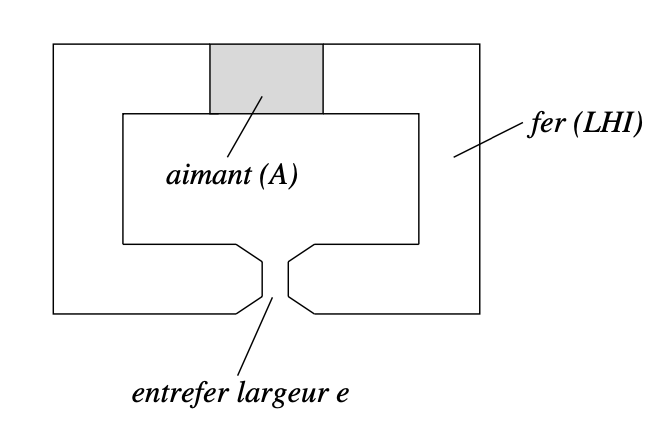
\includegraphics[scale=0.55]{entrefer.png}
   \end{minipage} \hfill
   \begin{minipage}[c]{.5\linewidth}
      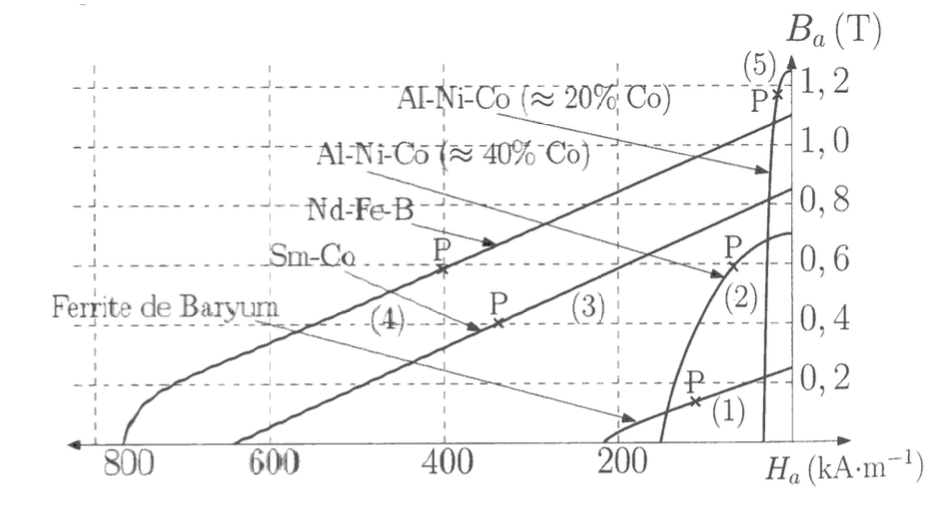
\includegraphics[scale=0.5]{caracteristique_ferro.png}
   \end{minipage}
\end{figure}

\begin{itemize}

	\item[$\heartsuit$] Économiquement, l’aimant ($A$) doit être dimensionné à volume minimal. Montrer qu’à volume $V_e$ et champ $B_e$ d’entrefer imposés, l’aimant le plus économique correspond à un produit d’énergie $|H_aB_a|$ maximal (critère d’Evershed). 
	
	On pourra faire l'hypothèse : $\frac{l_f}{\mu_{r,f}}\ll\frac{S_ae}{S_e}$

	\item[$\heartsuit$] Montrer que le produit d’énergie $|H_aB_a|$ d’un matériau dur est maximal quand on est au point $P$ d’Evershed, point de son quart de cycle $B_a(H)$ tel que le segment $PQ$ soit tangent à la courbe et le triangle $OPQ$ isocèle (Cf. figure).
	
	\begin{figure}[h!]
	\centering
		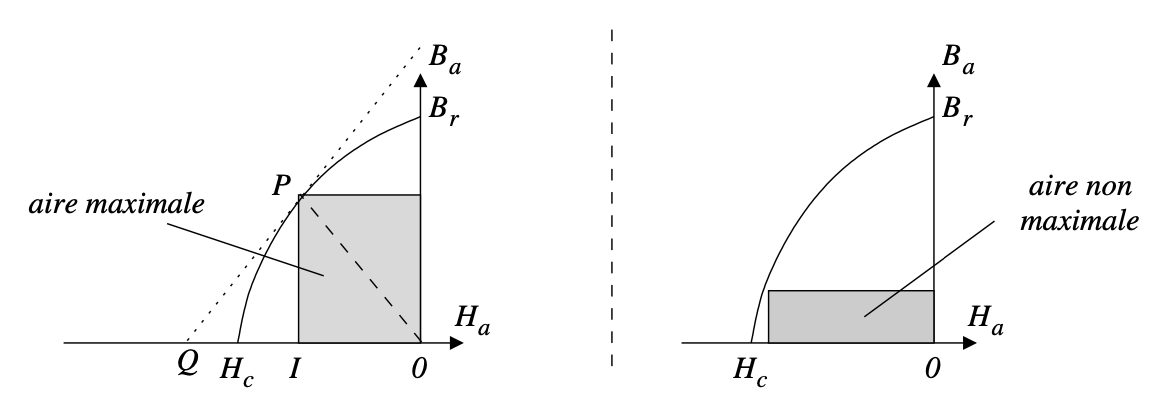
\includegraphics[scale=0.35]{produit_energie.png}
	\end{figure}	
	
	\item[$\heartsuit$] Dimensionner l'aimant ($A$) pour le samarium-cobalt Sm-Co. Données : $B_e$ =1.8T, $S_e$ =3.0cm$^2$, $e$=1.0cm, $l_f$=1.0m, $\mu_{r,f}=1,0\cdot10^4$.

\end{itemize}

\section*{Estimation de la puissance  dissipée dans un cycle hystérésis}

Un tore en acier de section 10cm$\times$12cm et de longueur 1.5m est enroulé par un bobinage dans lequel circule un courant à la fréquence $f=50$Hz, imposé par un générateur. L'acier est considéré comme un matériau ferromagnétique dur, de champ de saturation $B_{sat}=$1T, de champ rémanent $B_r=$0.7T et d'excitation coercitive $H_c=60$A/m.

Déterminer la puissance dégagée en moyenne lorsqu'on parcours cet hystéresis. Sous quelle forme se transforme l'énergie électrique apportée par le générateur ?

\section*{Transformateur réel série}

Un transformateur réel est représenté sur le schéma ci-dessous.

\begin{figure}[h!]
	\centering
		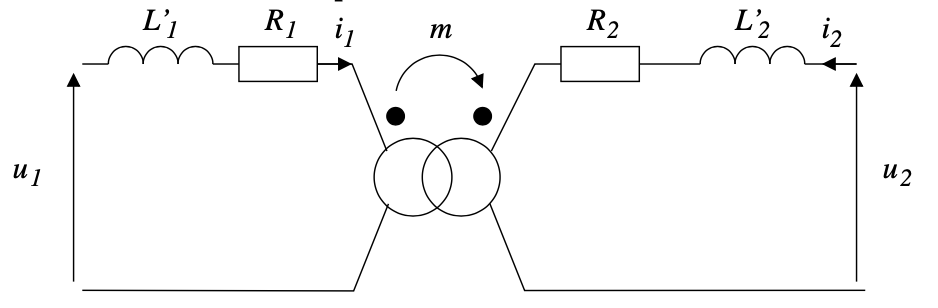
\includegraphics[scale=0.45]{transfo_reel.png}
\end{figure}	

Les résistances $R_1$ et $R_2$ représentent les résistances des fils de cuivre associées aux enroulements. Les inductances $L'_1$ et $L'_2$ sont des inductances de fuite modélisant les fuites de champ magnétique dues à la perméabilité finie du noyau.

\begin{itemize}
	
	\item[$\ast$] Montrer que le transformateur est équivalent au schéma suivant d’un transformateur idéal et d’une impédance $Z_{R_2}$ placée au secondaire. Donner son expression.
	
\begin{figure}[h!]
	\centering
		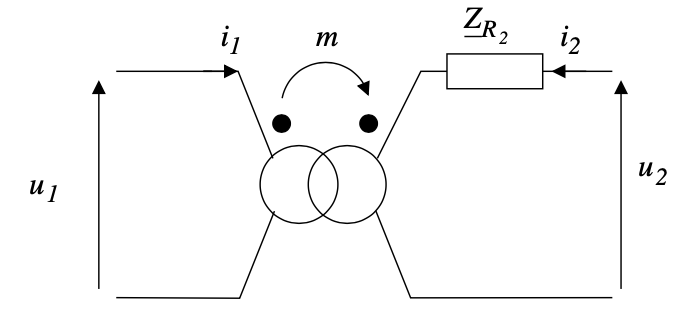
\includegraphics[scale=0.45]{transfo_reel2.png}
\end{figure}		
	
Les figures 1, 2 et 3 donnent les graphes liant amplitudes de tensions, de courants et de puissance moyenne appelée au primaire lorsque le secondaire est court-circuité à 50 Hz.	
	
\begin{figure}[h!]
	\centering
		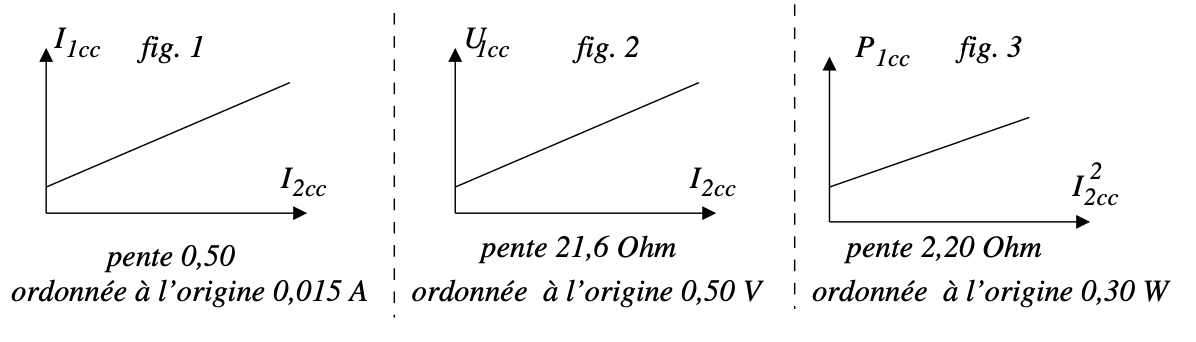
\includegraphics[scale=0.45]{courbe_transfo_reel.png}
\end{figure}		

	\item[$\ast$] Relier théoriquement $U_{1cc}$, $I_{2cc}$, $Z_{R_2}=Z_R$ et $m$, puis trouver une équation reliant théoriquement $P_{1cc}$ et $I_{2cc}$. Ces équations sont-elles en accord avec les courbes expérimentales ? Expliquer.

	\item[$\ast$] On a $R_2 =m R_1$ et $L'_2 =m L'_1$. Calculer numériquement $m$, $R1$, et $L1$.

\end{itemize}

\newpage

\section*{Transformateur réel}

On étudie un transformateur monophasé 220 V/110 V de puissance apparente 500 VA. Ce transformateur est alimenté au primaire en 220 V sous 50 Hz. Pour réaliser ce transformateur, on utilise le circuit magnétique représenté ci-dessous.

\begin{figure}[h!]
	\centering
		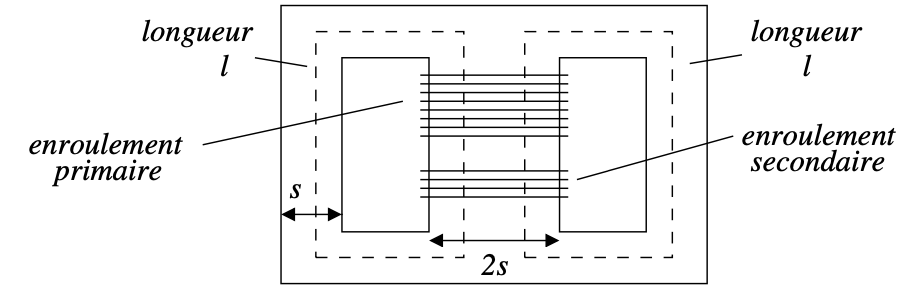
\includegraphics[scale=0.5]{transfo.png}
\end{figure}		

On admet que la section du tube d’induction est $s = 8.0 cm^2$ et que la longueur de la ligne de champ magnétique moyenne (en pointillé sur la figure) est $l = $25 cm.
Les tôles utilisées, non saturées, ont les caractéristiques suivantes : perméabilité
relative $\mu_r =3,1\cdot10^3$, masse volumique $\rho=7,2\cdot10^3$kg/m$^3$.

\begin{itemize}

	\item[$\triangleright$] Sachant que le primaire est alimenté par une tension de 220 V de fréquence 50 Hz, déterminer le nombre $N1$ de spires du primaire pour que, dans le fer, le champ magnétique soit de 1 tesla. En déduire $N_2$. Combien faudrait-il de spires si la fréquence valait 400 Hz ?

\end{itemize}

On cherche maintenant à représenter un modèle linéaire de ce transformateur réel tenant compte du caractère fini de la perméabilité relative $\mu_r$. On considère le schéma suivant pour le transformateur : on appelle $N_1$ le nombre de spires au primaire, $N_2$ le nombre de spires au secondaire, $\mu_r$ la perméabilité magnétique relative du milieu (non infinie !), $\phi$ le flux magnétique à travers la section droite $S$ du noyau. On appelle $l$ la longueur moyenne d’une ligne de champ dans le fer. On ne tient pas compte des pertes par effet Joule et des pertes fer.

\begin{figure}[h!]
	\centering
		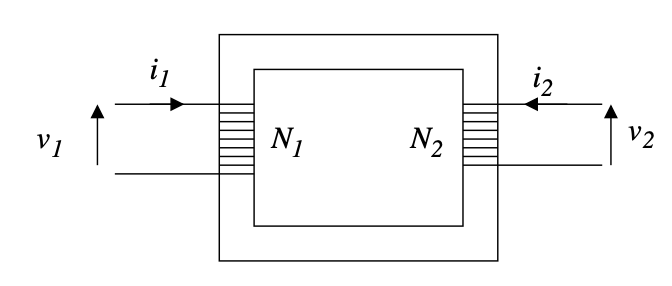
\includegraphics[scale=0.5]{transfo2.png}
\end{figure}		


\begin{itemize}

	\item[$\triangleright$] En se plaçant en régime forcé à la pulsation $\omega$, montrer que :
	\begin{align*}
		i_1-I_m=-\frac{N_2}{N_1}i_2
	\end{align*}
	avec $I_m=\frac{v_1}{j\omega L_1}$ le courant magnétisant, et $L_1$ l'inductance propre du circuit primaire, dont on donnera l'expression.
	
	\item[$\triangleright$] Que vaudrait $I_m$ pour $\mu_r\longrightarrow\infty$ ? Justifier alors le nouveau schéma proposé pour le transformateur pour tenir compte de ce courant magnétisant.

\begin{figure}[h!]
	\centering
		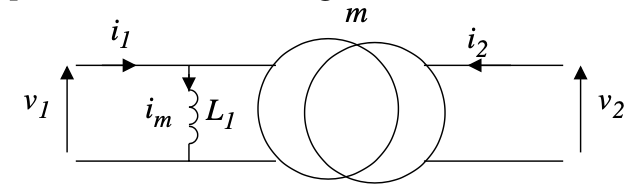
\includegraphics[scale=0.5]{transfo3.png}
\end{figure}		

	\item[$\triangleright$] Calculer la valeur efficace du courant magnétisant pour le transformateur réel étudié à la première question.

\end{itemize}

\newpage

\section*{Pic de courant dans un relais à palette}

On considère un convertisseur à mouvement linéaire, constitué d’un noyau (N) fixe en forme de U, d’une palette (P) cylindrique, tous deux en fer doux de section $S$. Ces deux parties forment un circuit magnétique d’entrefer $x(t)$ dont on considérera la canalisation parfaite des lignes de champ. Le fer doux est un matériau de grande perméabilité relative $\mu_r$.

La longueur moyenne totale de l’aimant en U et de la palette est notée $l$. La palette a une masse $m$.
Un bobinage (B) enroulé autour de (N) est, à partir de $t = 0$, alimenté par la tension continue U et parcouru par le courant $i(t)$. On note $R$ la résistance de l’enroulement constitué de $N$ spires.

\begin{figure}[h!]
	\centering
		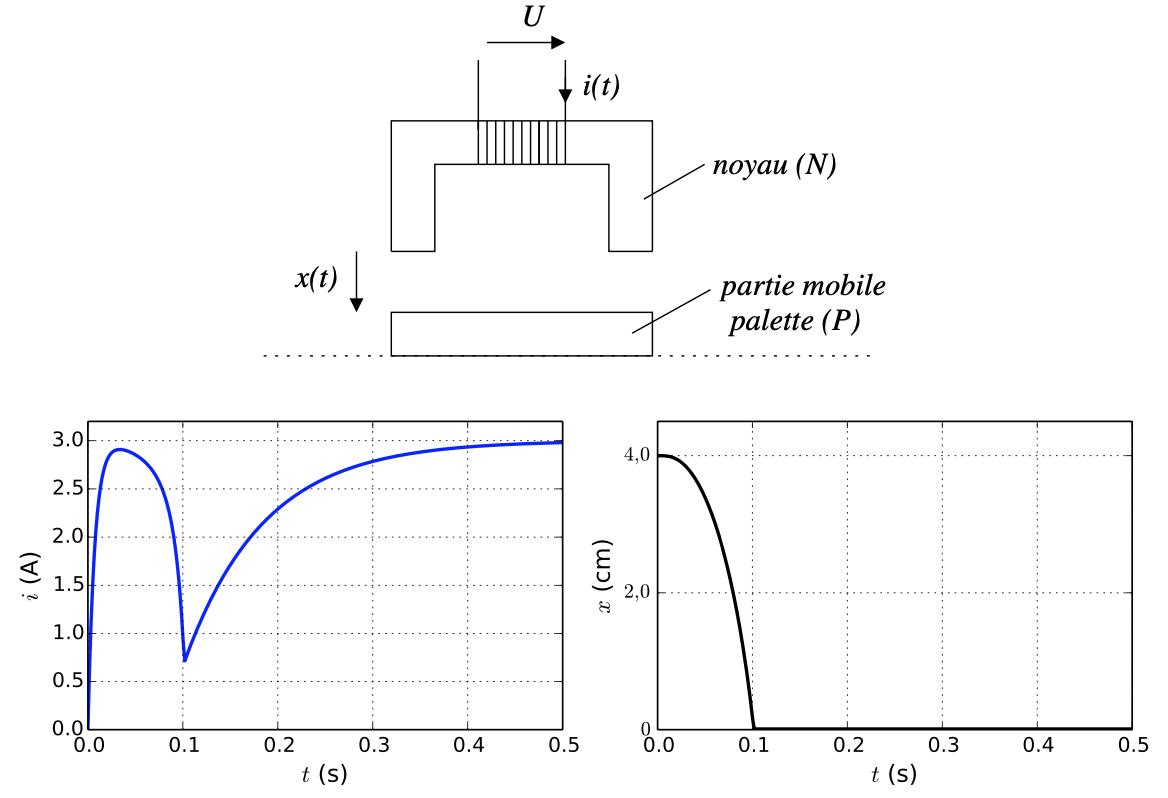
\includegraphics[scale=0.6]{relais.png}
\end{figure}		

Les figures ci-dessus donnent les courbes de simulation du courant et de la position de la palette au cours du temps. Paramètres : $U=30$V, $R=10\Omega$, $N=500$, $\mu_r=200$, $S=0,02$m$^2$, espacement initial $e=4$cm, $l=1,5$m, $m=10$kg.

\begin{itemize}
	
	\item[$\diamond$] Etablir le système d'équations différentielles satisfait par $i(t)$ et $x(t)$.
	
	\item[$\diamond$] Analyser les différentes phases du mouvement et expliquer l'allure des courbes.
	
\end{itemize}

\newpage

\section*{Transformateur à 3 bobinages}

Un transformateur à deux secondaires  possède trois enroulements, l'un de $N_{1}$ spires appelé primaire, et deux enroulements de $N_{2}$ et $N'_{2}$ spires appelés secondaires. On assimile la carcasse magnétique à un tore de section $S$ et de circonférence moyenne $L$.

On appelle $u_{1}$, $i_{1}$, $u_{2}$, $i_{2}$, $u'_{2}$ et $i'_{2}$ les tensions et intensités dans les différents enroulements.
\begin{center}
	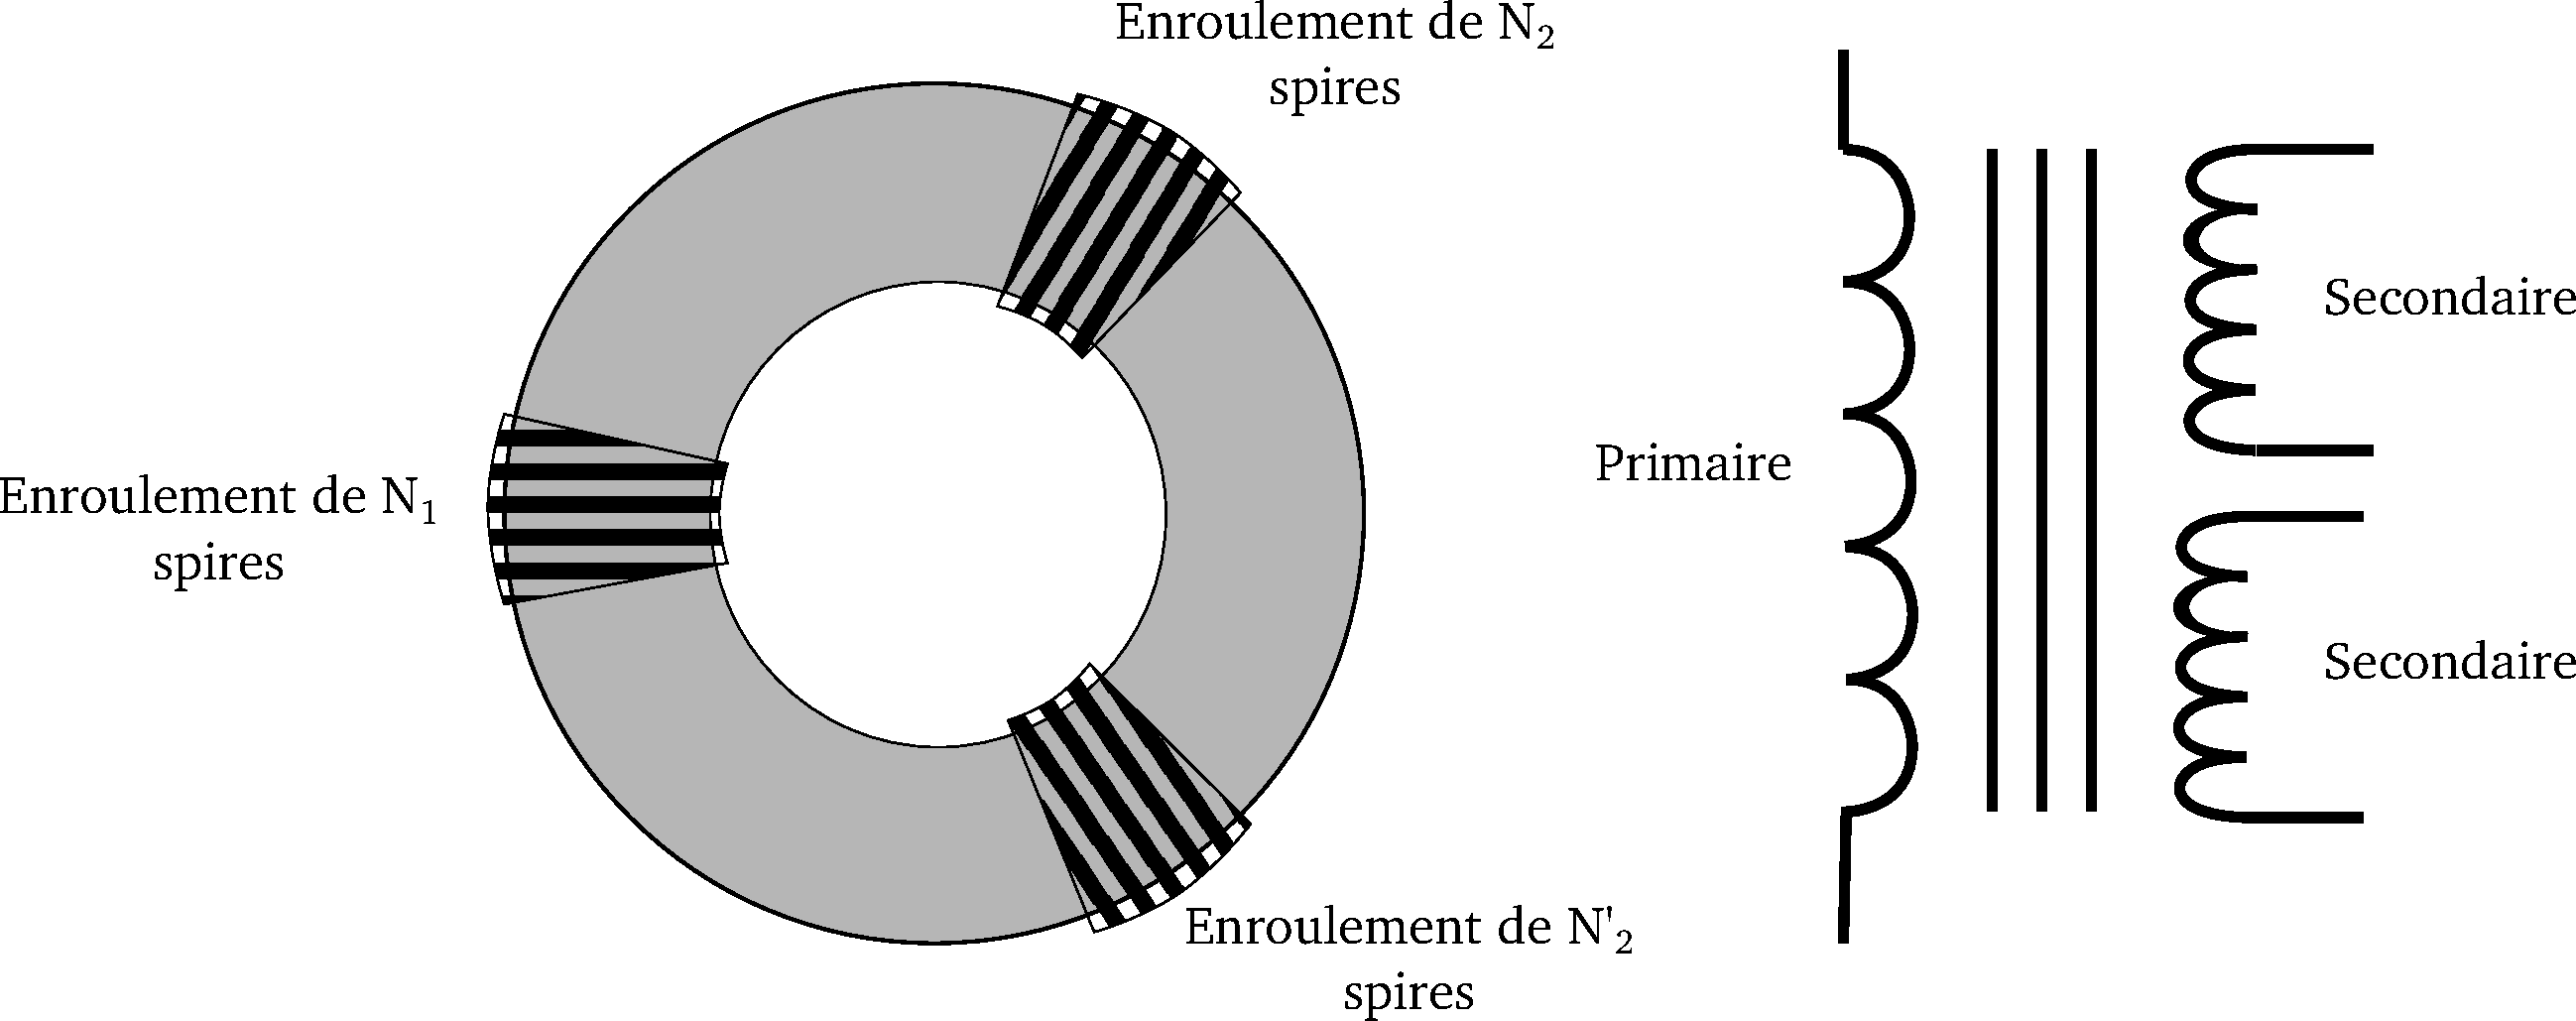
\includegraphics[scale=0.3]{transfo_3.pdf}
\end{center}

\begin{itemize}
	\item[$\clubsuit$] Déterminer la relation entre l'excitation magnétique moyenne dans la carcasse magnétique et les paramètres électriques dans les enroulements. Faire de même pour les relations entre le flux à travers une spire et les paramètres du circuit.
	
	\item[$\clubsuit$] En déduire, dans le cas du transformateur parfait, les relations entre tensions et intensités. Donner une modélisation à l'aide de transformateurs idéaux de ce transformateur parfait.	
\end{itemize}

\section*{Transfert de puissance}

On souhaite alimenter un dipôle ohmique de résistance $R$ par un générateur sinusoïdal de fem $e(t) = E_{0} cos(\omega t)$ par l'intermédiaire d'un transformateur supposé parfait de rapport de transmission $m$. Les câbles électriques reliant le transformateur ont un coefficient d'auto-induction $L$ et l'ensemble générateur-fils une résistance $r$.

\begin{itemize}
	\item[$\bigstar$] Déterminer le rapport de transformation pour avoir la puissance maximale dissipée dans $R$.
	\item[$\bigstar$] Calculer le rendement de l'installation électrique en fonction de $m$.
	\item[$\bigstar$] Tracer les courbes de la puissance dissipée dans $R$ et du rendement en fonction de $m$.
\end{itemize}

\end{document}